\documentclass[10pt,a4paper]{article}

\usepackage[utf8]{inputenc}
\usepackage[T1]{fontenc}
\usepackage{lmodern}
\renewcommand{\figurename}{Figura}
\renewcommand{\tablename}{Tabela}
\usepackage{microtype}
\usepackage[top=1.5cm,bottom=1.5cm,left=1.6cm,right=1.6cm]{geometry}
\usepackage{amsmath,amssymb}
\usepackage{booktabs}
\usepackage{tabularx}
\usepackage{array}
\usepackage{enumitem}
\usepackage{xcolor}
\usepackage{tikz}
\usetikzlibrary{shapes.geometric, arrows.meta, positioning, fit, backgrounds, calc}
\usepackage{fancyhdr}
\usepackage{titlesec}
\usepackage{hyperref}

% Paleta de cores sóbria e acadêmica
\definecolor{ufsblue}{HTML}{0B4F6C}
\definecolor{ufslate}{HTML}{2C3E50}
\definecolor{ufsgreen}{HTML}{1B7A43}
\definecolor{ufsorange}{HTML}{B85D19}
\definecolor{lightgray}{HTML}{F4F6F8}
\definecolor{bordergray}{HTML}{D0D7DE}

\hypersetup{
    colorlinks=true,
    linkcolor=ufsblue,
    urlcolor=ufsblue,
    citecolor=ufsblue,
    pdftitle={Relatório Técnico - DComp Drive - Sistemas Distribuídos (COMP0470)},
    pdfauthor={Equipe DComp Drive - UFS}
}

% Ajustes de espaçamento para manter 6-7 páginas densas e bem diagramadas
\setlength{\parindent}{0pt}
\setlength{\parskip}{3.2pt}
\setlist[itemize]{noitemsep, topsep=1.5pt, leftmargin=1.4em}
\setlist[enumerate]{noitemsep, topsep=1.5pt, leftmargin=1.5em}

\titleformat{\section}
  {\normalfont\large\bfseries\color{ufsblue}}{\thesection.}{0.5em}{}[\titlerule]
\titlespacing*{\section}{0pt}{8pt}{4pt}

\titleformat{\subsection}
  {\normalfont\normalsize\bfseries\color{ufslate}}{\thesubsection}{0.5em}{}
\titlespacing*{\subsection}{0pt}{6pt}{2pt}

\titleformat{\subsubsection}
  {\normalfont\normalsize\itshape\bfseries\color{ufslate}}{\thesubsubsection}{0.5em}{}
\titlespacing*{\subsubsection}{0pt}{4pt}{2pt}

% Cabeçalho e rodapé
\pagestyle{fancy}
\fancyhf{}
\fancyhead[L]{\footnotesize\textcolor{ufslate}{\textbf{DComp Drive} — Sistema Distribuído de Armazenamento de Arquivos}}
\fancyhead[R]{\footnotesize\textcolor{ufslate}{UFS • COMP0470 — Sistemas Distribuídos}}
\fancyfoot[C]{\footnotesize\thepage}
\renewcommand{\headrulewidth}{0.4pt}
\renewcommand{\footrulewidth}{0pt}

\newcolumntype{Y}{>{\raggedright\arraybackslash}X}

\begin{document}

% =====================================================================
% CABEÇALHO DO RELATÓRIO TÉCNICO
% =====================================================================
\begin{center}
    {\large\bfseries UNIVERSIDADE FEDERAL DE SERGIPE (UFS)}\\
    {\normalsize DEPARTAMENTO DE COMPUTAÇÃO (DCOMP) — COMP0470: SISTEMAS DISTRIBUÍDOS}\\
    {\small Prof. Rafael Oliveira Vasconcelos}\\[8pt]
    {\LARGE\bfseries\color{ufsblue} DComp Drive: Projeto e Implementação de um Sistema Distribuído de Armazenamento de Arquivos Tolerante a Falhas}\\[4pt]
    {\normalsize\itshape Relatório Técnico — Parte 1: Arquitetura, Protocolos, Replicação, Consistência e Segurança}
\end{center}
\vspace{-4pt}
\noindent\rule{\textwidth}{0.8pt}
\vspace{2pt}

\textbf{Resumo.} Este relatório técnico apresenta as decisões arquiteturais, os protocolos de comunicação, a modelagem de metadados e os algoritmos distribuídos implementados no \textbf{DComp Drive}, um sistema distribuído de armazenamento de arquivos orientado a blocos inspirado em arquiteturas como HDFS, Google File System (GFS), Ceph e MinIO. O sistema desacopla estritamente o \textit{Plano de Controle} (gerenciamento hierárquico de diretórios, alocação multicritério de réplicas, controle de concorrência via \textit{leases}, detecção de falhas por \textit{heartbeats} e fila priorizada de re-replicação) do \textit{Plano de Dados} (transferência paralela de blocos em \textit{streaming} diretamente entre clientes e nós de armazenamento e cópia direta nó-a-nó). A solução garante integridade ponta a ponta via hashes \texttt{SHA-256} com validação em escrita, leitura e varredura periódica em segundo plano (\textit{scrubbing}), além de oferecer criptografia autenticada opcional no cliente (\texttt{AES-256-GCM}).

\noindent\rule{\textwidth}{0.4pt}

% =====================================================================
% 1. ARQUITETURA E DIAGRAMA DOS COMPONENTES
% =====================================================================
\section{Arquitetura do Sistema e Separação de Planos}

O \textbf{DComp Drive} adota uma arquitetura distribuída assimétrica baseada na separação estrita entre o \textbf{Plano de Controle} (\textit{Control Plane}) e o \textbf{Plano de Dados} (\textit{Data Plane}), evitando que o servidor de metadados se torne um gargalo de largura de banda ou de processamento criptográfico durante a transferência de arquivos. A Figura~\ref{fig:arquitetura} ilustra a topologia dos componentes e os fluxos de controle e dados.

\begin{figure}[htbp]
\centering
\resizebox{\textwidth}{!}{%
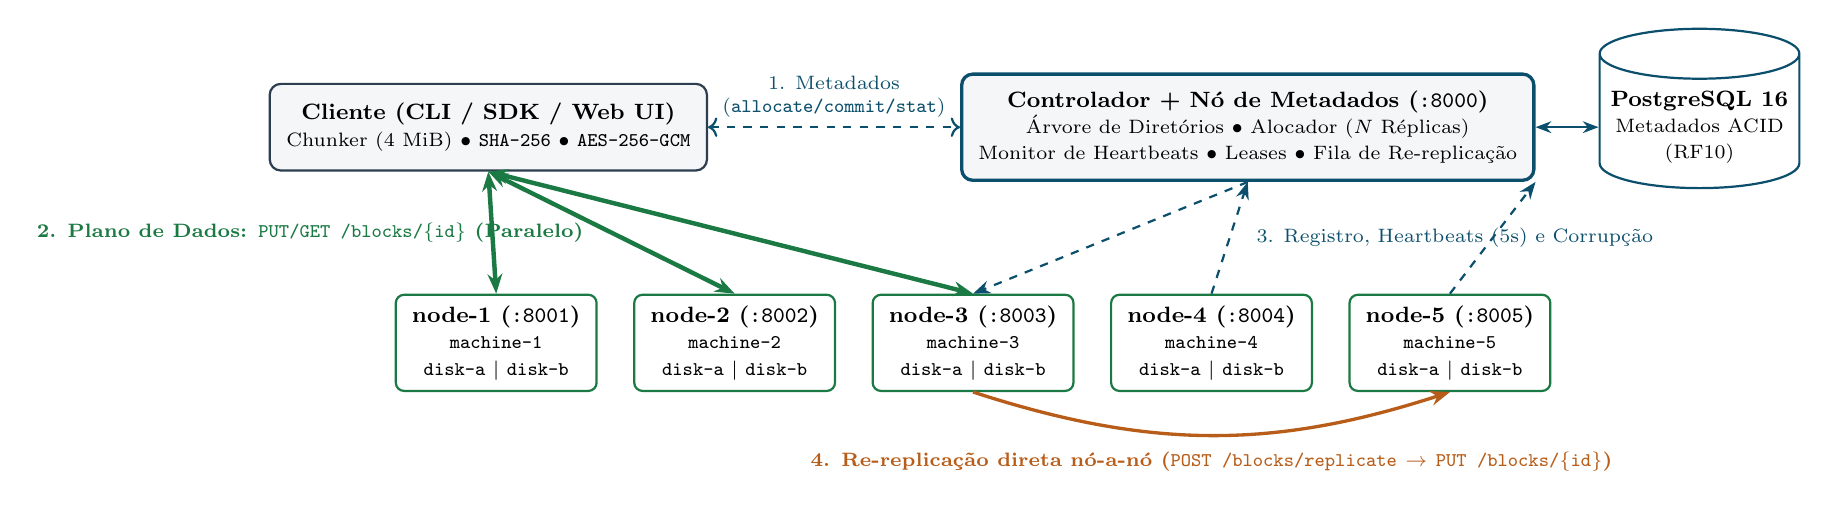
\begin{tikzpicture}[
    font=\footnotesize,
    node distance=0.8cm and 1.0cm,
    box/.style={rectangle, rounded corners=4pt, draw=ufslate, thick, fill=white, align=center, minimum height=1.1cm, inner sep=6pt},
    ctrlbox/.style={rectangle, rounded corners=4pt, draw=ufsblue, very thick, fill=lightgray, align=center, minimum height=1.2cm, inner sep=6pt},
    dbbox/.style={cylinder, shape border rotate=90, aspect=0.25, draw=ufsblue, thick, fill=white, align=center, minimum height=1.1cm, minimum width=2.2cm, inner sep=4pt},
    nodebox/.style={rectangle, rounded corners=3pt, draw=ufsgreen, thick, fill=white, align=center, minimum height=1.05cm, minimum width=2.55cm, inner sep=4pt},
    ctrlarrow/.style={-{Stealth[length=2.2mm]}, thick, color=ufsblue, dashed},
    dataarrow/.style={<->, >={Stealth[length=2.5mm]}, ultra thick, color=ufsgreen},
    replarrow/.style={-{Stealth[length=2.5mm]}, very thick, color=ufsorange}
]

    % Cliente
    \node[box, minimum width=4.6cm, fill=lightgray] (client) {
        \textbf{Cliente (CLI / SDK / Web UI)}\\
        \scriptsize Chunker ($4\text{ MiB}$) $\bullet$ \texttt{SHA-256} $\bullet$ \texttt{AES-256-GCM}
    };

    % Controlador
    \node[ctrlbox, right=3.2cm of client, minimum width=5.2cm] (controller) {
        \textbf{Controlador + Nó de Metadados (\texttt{:8000})}\\
        \scriptsize Árvore de Diretórios $\bullet$ Alocador ($N$ Réplicas)\\
        \scriptsize Monitor de Heartbeats $\bullet$ Leases $\bullet$ Fila de Re-replicação
    };

    % PostgreSQL
    \node[dbbox, right=0.8cm of controller] (postgres) {
        \textbf{PostgreSQL 16}\\
        \scriptsize Metadados ACID\\
        \scriptsize (RF10)
    };

    % Storage Nodes
    \node[nodebox, below=1.55cm of client, xshift=0.1cm] (n1) {
        \textbf{node-1 (\texttt{:8001})}\\
        \scriptsize \texttt{machine-1}\\
        \scriptsize \texttt{disk-a} $|$ \texttt{disk-b}
    };
    \node[nodebox, right=0.45cm of n1] (n2) {
        \textbf{node-2 (\texttt{:8002})}\\
        \scriptsize \texttt{machine-2}\\
        \scriptsize \texttt{disk-a} $|$ \texttt{disk-b}
    };
    \node[nodebox, right=0.45cm of n2] (n3) {
        \textbf{node-3 (\texttt{:8003})}\\
        \scriptsize \texttt{machine-3}\\
        \scriptsize \texttt{disk-a} $|$ \texttt{disk-b}
    };
    \node[nodebox, right=0.45cm of n3] (n4) {
        \textbf{node-4 (\texttt{:8004})}\\
        \scriptsize \texttt{machine-4}\\
        \scriptsize \texttt{disk-a} $|$ \texttt{disk-b}
    };
    \node[nodebox, right=0.45cm of n4] (n5) {
        \textbf{node-5 (\texttt{:8005})}\\
        \scriptsize \texttt{machine-5}\\
        \scriptsize \texttt{disk-a} $|$ \texttt{disk-b}
    };

    % Conexões
    \draw[ctrlarrow, <->] (client.east) -- node[above, align=center, font=\scriptsize\color{ufsblue}] {1. Metadados\\(\texttt{allocate/commit/stat})} (controller.west);
    \draw[<->, >={Stealth[length=2mm]}, thick, color=ufsblue] (controller.east) -- (postgres.west);

    % Plano de dados Cliente <-> Storage Nodes
    \draw[dataarrow] (client.south) -- node[left, xshift=-6pt, font=\scriptsize\bfseries\color{ufsgreen}] {2. Plano de Dados: \texttt{PUT/GET /blocks/\{id\}} (Paralelo)} (n2.north);
    \draw[dataarrow] (client.south) -- (n1.north);
    \draw[dataarrow] (client.south) -- (n3.north);

    % Heartbeats e ordens do Controlador
    \draw[ctrlarrow] (n4.north) -- node[right, xshift=6pt, font=\scriptsize\color{ufsblue}] {3. Registro, Heartbeats (5s) e Corrupção} (controller.south);
    \draw[ctrlarrow] (controller.south) -- (n3.north);
    \draw[ctrlarrow] (n5.north) -- (controller.south east);

    % Cópia nó a nó
    \draw[replarrow, bend right=18] (n3.south) to node[below, yshift=-2pt, font=\scriptsize\bfseries\color{ufsorange}] {4. Re-replicação direta nó-a-nó (\texttt{POST /blocks/replicate} $\rightarrow$ \texttt{PUT /blocks/\{id\}})} (n5.south);

\end{tikzpicture}%
}
\caption{Arquitetura do DComp Drive destacando a separação entre o Plano de Controle (tracejado azul), o Plano de Dados cliente-nó (verde) e o fluxo de recuperação direta nó-a-nó (laranja).}
\label{fig:arquitetura}
\end{figure}

\subsection{Papéis Arquiteturais e Acúmulo de Funções}
Conforme permitido pela especificação, os quatro papéis fundamentais do sistema foram distribuídos em três componentes executáveis independentes:

\begin{enumerate}
    \item \textbf{Controlador + Nó de Metadados (Processos Unificados — \texttt{src/controller/}):} O processo central acumula deliberadamente os papéis de \textit{Controlador de Cluster} e de \textit{Nó de Metadados}. Essa unificação elimina a necessidade de transações distribuídas (2PC) entre o catálogo de arquivos e o gerenciador de blocos: em uma única transação relacional no PostgreSQL, o serviço valida a hierarquia de diretórios, adquire o \textit{lease} de concorrência, consulta o espaço livre reportado pelos últimos \textit{heartbeats} e persiste o plano de alocação das réplicas. O componente jamais recebe ou retransmite o conteúdo binário dos arquivos no fluxo da CLI.
    \item \textbf{Nó de Armazenamento (\textit{Storage Node} — \texttt{src/storage\_node/}):} Processo autônomo responsável pelo plano de dados físico. Cada nó gerencia múltiplos diretórios locais configurados via \texttt{DISK\_MOUNTS} que simulam discos independentes (\texttt{disk-a}, \texttt{disk-b}). Suas responsabilidades incluem: persistir e servir blocos binários em \textit{streaming}; validar hashes \texttt{SHA-256} em tempo real na escrita e antes de cada leitura; executar a rotina periódica de \textit{scrubbing}; reportar anomalias ao controlador; enviar \textit{heartbeats} periódicos com telemetria de capacidade (\texttt{shutil.disk\_usage}) e executar cópias diretas para outros nós na re-replicação.
    \item \textbf{Cliente (\texttt{src/client/}):} Disponibilizado como interface de linha de comando (\texttt{Typer} + \texttt{Rich}), biblioteca assíncrona (\texttt{DriveClient}) e painel Web integrado (\texttt{/drive}). O cliente particiona arquivos em blocos (\textit{chunks}), realiza opcionalmente a cifra autenticada \texttt{AES-256-GCM}, computa os hashes \texttt{SHA-256} (de cada bloco e do arquivo completo) e executa transferências paralelas diretamente contra os Nós de Armazenamento utilizando \texttt{httpx}.
\end{enumerate}

\subsection{Justificativa da Stack Tecnológica}
O sistema foi desenvolvido em \textbf{Python 3.11+} com arquitetura 100\% assíncrona baseada em \textbf{\texttt{asyncio}}, \textbf{\texttt{FastAPI}} e \textbf{\texttt{Uvicorn}}. Para a comunicação entre componentes, optou-se por uma \textbf{API REST sobre HTTP/1.1}:
\begin{itemize}
    \item \textbf{Plano de Controle (\texttt{application/json}):} Requisições de metadados, registro, \textit{heartbeat} e relatórios de estado são validadas rigorosamente por contratos \textbf{\texttt{Pydantic v2}} compartilhados em \texttt{src/common/schemas.py}.
    \item \textbf{Plano de Dados (\texttt{application/octet-stream}):} O envio e a leitura de blocos utilizam \textit{HTTP Streaming} assíncrono (\texttt{request.stream()} e \texttt{StreamingResponse}) com blocos de leitura em memória limitados a \texttt{BUFFER\_SIZE = 1 MiB}, permitindo transferir arquivos grandes com consumo constante de RAM.
    \item \textbf{Persistência Relacional (\texttt{PostgreSQL 16} + \texttt{SQLAlchemy 2.0 Async} + \texttt{asyncpg}):} Atende ao requisito \textbf{RF10} garantindo durabilidade ACID e integridade referencial. Se o controlador reiniciar ou sofrer queda, todo o estado da árvore de diretórios, blocos, réplicas e nós é recuperado instantaneamente do banco sem intervenção manual.
    \item \textbf{Orquestração Reproduzível (\texttt{Docker} + \texttt{Docker Compose}):} O ambiente padrão sobe 7 contêineres isolados: 1 instância do PostgreSQL 16 (mapeada na porta \texttt{5433} do host para evitar colisão com bancos locais), 1 Controlador (\texttt{:8000}) e 5 Nós de Armazenamento (\texttt{:8001} a \texttt{:8005}), cada um associado a um \texttt{MACHINE\_ID} distinto (\texttt{machine-1..5}) e montando 2 volumes Docker dedicados (\texttt{/data/disk\_a} e \texttt{/data/disk\_b}), totalizando 10 discos monitorados.
\end{itemize}

% =====================================================================
% 2. MODELAGEM DE DADOS E PROTOCOLOS DE COMUNICAÇÃO
% =====================================================================
\section{Modelagem de Metadados, Protocolos e Fluxos de Operação}

\subsection{Esquema Relacional de Metadados e Persistência (RF10)}
O banco de dados do Nó de Metadados (\texttt{src/controller/models.py}) é estruturado em cinco tabelas relacionais com exclusão em cascata (\texttt{ON DELETE CASCADE}) e restrições de unicidade que impedem violações de replicação no próprio nível de armazenamento de metadados:

\begin{table}[htbp]
\centering
\footnotesize
\renewcommand{\arraystretch}{1.15}
\begin{tabularx}{\textwidth}{l l Y}
\toprule
\textbf{Tabela} & \textbf{Chave Primária / Constraints} & \textbf{Atributos e Papel no Sistema} \\
\midrule
\texttt{storage\_nodes} & \texttt{PK (node\_id)} & Armazena \texttt{host\_url}, \texttt{machine\_id} (indexado), \texttt{status} (\texttt{ALIVE}, \texttt{SUSPECT}, \texttt{DEAD}, \texttt{DRAINING}) e \texttt{last\_heartbeat} (UTC). \\
\texttt{node\_disks} & \texttt{PK (disk\_id)}, \texttt{FK (node\_id)} & Mapeia cada diretório físico (\texttt{mount\_path}), capacidade (\texttt{total\_bytes}, \texttt{used\_bytes}) e flag \texttt{is\_active}. Calcula dinamicamente \texttt{free\_bytes} e \texttt{usage\_pct}. \\
\texttt{entries} & \texttt{PK (entry\_id)}, \texttt{UNIQUE (path)} & Representa arquivos e diretórios. Guarda \texttt{parent\_path}, \texttt{is\_dir}, \texttt{size\_bytes}, \texttt{file\_hash} (\texttt{SHA-256} em texto claro), \texttt{replication\_target} ($N$), \texttt{is\_encrypted}, \texttt{status} (\texttt{DIRECTORY}, \texttt{WRITING}, \texttt{HEALTHY}, \texttt{SUB\_REPLICATED}, \texttt{RECOVERING}, \texttt{CORRUPTED}) e \texttt{lease\_expires\_at}. \\
\texttt{blocks} & \texttt{PK (block\_id)}, \texttt{UNIQUE (entry\_id, block\_index)} & Metadados de cada \textit{chunk}: \texttt{block\_index} ($0, 1, \dots$), \texttt{size\_bytes} (tamanho de rede), \texttt{block\_hash} (\texttt{SHA-256} dos bytes de rede) e \texttt{encryption\_nonce} (24 hex chars). \\
\texttt{block\_replicas} & \texttt{PK (block\_id, disk\_id)}, \texttt{UNIQUE (block\_id, node\_id)} & Localização física de cada cópia (\texttt{node\_id}, \texttt{disk\_id}) e seu estado (\texttt{PENDING}, \texttt{VERIFIED}, \texttt{COPYING}, \texttt{CORRUPTED}). As constraints garantem no SGBD que um bloco \textbf{jamais} tenha duas réplicas no mesmo disco ou no mesmo nó. \\
\bottomrule
\end{tabularx}
\caption{Modelagem relacional persistida no PostgreSQL 16 (\texttt{src/controller/models.py}).}
\label{tab:schema}
\end{table}

\subsection{Contratos de Mensagens e Rotas da API}
A Tabela~\ref{tab:api} sintetiza os contratos de comunicação REST entre Cliente, Controlador e Nós de Armazenamento.

\begin{table}[!htbp]
\centering
\footnotesize
\renewcommand{\arraystretch}{1.1}
\begin{tabularx}{\textwidth}{l l l Y}
\toprule
\textbf{Alvo} & \textbf{Método e Rota} & \textbf{Formato} & \textbf{Semântica e Parâmetros Principais} \\
\midrule
Controlador & \texttt{POST /nodes/register} & JSON & Registro ativo e reconciliação de inventário (\texttt{existing\_blocks} $\rightarrow$ \texttt{obsolete\_blocks}). \\
Controlador & \texttt{POST /nodes/heartbeat} & JSON & Atualiza \texttt{last\_heartbeat} e telemetria de discos (\texttt{total\_bytes}, \texttt{used\_bytes}). \\
Controlador & \texttt{POST /nodes/\{id\}/drain} & JSON & Marca nó como \texttt{DRAINING} e agenda migração de suas réplicas para nós \texttt{ALIVE}. \\
Controlador & \texttt{POST /files/allocate} & JSON & Cria \textit{lease} \texttt{WRITING} e retorna $N$ destinos (\texttt{node\_id, host\_url, disk\_id}) por bloco. \\
Controlador & \texttt{POST /files/commit} & JSON & Valida quórum $W$ de réplicas confirmadas, remove \texttt{PENDING} restantes e libera o \textit{lease}. \\
Controlador & \texttt{GET /files/metadata} & JSON & Retorna metadados, hash e réplicas (\texttt{for\_read=true} bloqueia se \texttt{WRITING} com \texttt{HTTP 409}). \\
Controlador & \texttt{POST|GET /dirs} & JSON & Criação (\texttt{mkdir -p}) e listagem de diretórios (\texttt{ls}) com recálculo dinâmico de saúde. \\
Controlador & \texttt{PATCH /entries/move} & JSON & Renomeia ou move arquivo ou subárvore completa de diretório (\texttt{mv}) atomicamente. \\
Controlador & \texttt{DELETE /entries} & JSON & Remove entrada/subárvore do banco e dispara deleção física assíncrona nos nós (\texttt{rm}). \\
Controlador & \texttt{POST /blocks/report-corruption} & JSON & Descarta réplica corrompida, apaga arquivo físico e dispara cópia substituta imediata. \\
Controlador & \texttt{GET /cluster/status} e \texttt{/metrics} & JSON & Visibilidade do cluster (nós por estado, discos, arquivos por estado e re-replicações ativas). \\
\midrule
Storage Node & \texttt{PUT /blocks/\{id\}} & Stream &Query: \texttt{disk\_id, expected\_hash}. Valida \texttt{SHA-256} em streaming e publica \texttt{.blk} + \texttt{.sha256}. \\
Storage Node & \texttt{GET /blocks/\{id\}} & Stream &Query: \texttt{disk\_id}. Recalcula \texttt{SHA-256} antes do 1º byte; se inválido, reporta e retorna \texttt{422}. \\
Storage Node & \texttt{DELETE /blocks/\{id\}} & HTTP 204 &Query: \texttt{disk\_id}. Remove \texttt{\{id\}.blk} e \texttt{\{id\}.sha256} com \texttt{fsync} no diretório pai. \\
Storage Node & \texttt{POST /blocks/replicate} & JSON & Ordem de cópia nó-a-nó: valida destino no controlador e faz \texttt{PUT} direto ao nó alvo. \\
\bottomrule
\end{tabularx}
\caption{Protocolos e endpoints de comunicação dos Planos de Controle e de Dados.}
\label{tab:api}
\end{table}

\subsection{Fluxo de Escrita Paralela, Leitura com Fallback e Armazenamento Físico}
\textbf{Fluxo de Escrita (\texttt{put}):}
\begin{enumerate}
    \item \textbf{Preparação em Spool Local:} Antes de contatar o controlador, o cliente (\texttt{prepare\_file} em \texttt{src/client/chunker.py}) lê o arquivo de origem em blocos de \texttt{chunk\_size\_mb} ($4\text{ MiB}$), atualiza o \texttt{SHA-256} do texto claro completo (\texttt{file\_hash}), cifra opcionalmente cada bloco com \texttt{AES-256-GCM} gerando um \texttt{nonce} único de 12 bytes, calcula o \texttt{SHA-256} dos bytes de rede (\texttt{block\_hash}) e grava um \textit{snapshot} temporário local. Isso garante que arquivos grandes não consumam o tempo do \textit{lease} do servidor com processamento local de hash/cifra.
    \item \textbf{Alocação e Lease:} O cliente envia \texttt{POST /files/allocate}. O controlador cria a entrada em estado \texttt{WRITING} com expiração \texttt{lease\_expires\_at}, seleciona $N$ destinos distintos por bloco, cria registros \texttt{BlockReplica} em estado \texttt{PENDING} e retorna o plano de alocação junto com o quórum de escrita exigido ($W$).
    \item \textbf{Transferência Paralela em Streaming:} O cliente abre tarefas assíncronas paralelas (controladas por semáforo de concorrência) e envia cada bloco diretamente aos $N$ Nós de Armazenamento via \texttt{PUT /blocks/\{block\_id\}}.
    \item \textbf{Publicação Atômica no Nó:} O \texttt{DiskManager} (\texttt{src/storage\_node/disk\_manager.py}) grava o stream recebido em um arquivo temporário \texttt{*.blk.tmp} no mesmo volume de destino enquanto calcula o \texttt{SHA-256}. Se o hash final divergir de \texttt{expected\_hash}, o arquivo temporário é removido no bloco \texttt{finally} e retorna-se \texttt{HTTP 422}. Se coincidir, o nó executa \texttt{flush()} e \texttt{os.fsync()} no descritor do arquivo, grava atomicamente o arquivo auxiliar \texttt{<block\_id>.sha256} e publica o bloco final via \texttt{os.replace()} seguido de \texttt{fsync} no diretório POSIX.
    \item \textbf{Quórum $W$ e Commit:} Assim que $W$ réplicas de um bloco respondem \texttt{201 Created}, o cliente não precisa aguardar um eventual nó lento (\texttt{asyncio.FIRST\_COMPLETED}): ele cancela as esperas excedentes daquele bloco e, uma vez atingido o quórum para todos os blocos, envia \texttt{POST /files/commit}. O controlador promove as réplicas confirmadas para \texttt{VERIFIED}, remove do banco as réplicas \texttt{PENDING} não confirmadas (agendando deleção física assíncrona nos nós correspondentes) e transiciona o arquivo para \texttt{HEALTHY} (se todas as $N$ réplicas foram confirmadas) ou \texttt{SUB\_REPLICATED} (se $W \le \text{confirmadas} < N$, deixando que o monitor complete as cópias faltantes em background).
\end{enumerate}

\textbf{Fluxo de Leitura com Fallback e Auto-Recuperação (\texttt{get}):}
\begin{enumerate}
    \item O cliente consulta \texttt{GET /files/metadata?path=...\&for\_read=true}. O controlador retorna apenas réplicas \texttt{VERIFIED} localizadas em nós \texttt{ALIVE} ou \texttt{DRAINING} (ordenadas priorizando nós \texttt{ALIVE}).
    \item Para cada bloco, o cliente tenta baixar da primeira réplica via \texttt{GET /blocks/\{block\_id\}}. No Nó de Armazenamento, o método \texttt{open\_verified} lê o arquivo \texttt{.blk} para um \texttt{SpooledTemporaryFile} verificando o \texttt{SHA-256} completo contra o sidecar \texttt{.sha256} \textbf{antes de transmitir o primeiro byte}. Caso detecte corrupção em disco (\textit{bit rot}), o próprio nó aciona \texttt{POST /blocks/report-corruption} no controlador e responde \texttt{HTTP 422}.
    \item O cliente também recalcula o \texttt{SHA-256} e valida o tamanho exato dos bytes recebidos pela rede. Se ocorrer falha de conexão, erro HTTP ou divergência de hash, o cliente reporta a corrupção ao controlador (em caso de falha de integridade), descarta os bytes inválidos e faz \textbf{fallback transparente} para a próxima réplica saudável do bloco.
    \item Após baixar e (se aplicável) decifrar todos os blocos em um arquivo temporário \texttt{.<nome>.part} na pasta de destino, o cliente recalcula o \texttt{SHA-256} do arquivo reconstruído completo, compara com \texttt{file\_hash}, executa \texttt{fsync} e publica o arquivo final atomicamente com \texttt{os.replace()}. Assim, uma leitura jamais sobrescreve ou corrompe um arquivo local preexistente se todas as réplicas falharem ou se a chave de criptografia estiver incorreta.
\end{enumerate}

% =====================================================================
% 3. POSICIONAMENTO, DETECÇÃO DE FALHAS E RE-REPLICAÇÃO
% =====================================================================
\section{Algoritmos de Posicionamento, Detecção de Falhas e Re-replicação}

\subsection{Descoberta Automática, Reconciliação e Máquina de Estados de Falha (RF5, RF6)}
Os Nós de Armazenamento descobrem e ingressam no cluster sem necessidade de editar listas estáticas no controlador nem reiniciar o sistema. Ao iniciar, o \texttt{NodeAgent} (\texttt{src/storage\_node/workers.py}) executa \texttt{verified\_inventory()}, que inspeciona todos os discos locais e inclui apenas os blocos cujo par \texttt{.blk}/\texttt{.sha256} passa pela verificação criptográfica local, enviando-os em \texttt{POST /nodes/register}. Além disso, caso o controlador seja reiniciado com banco limpo e responda \texttt{HTTP 404} a um \textit{heartbeat}, o nó limpa automaticamente seu evento de registro e reexecuta o protocolo completo de registro e reconciliação.

\textbf{Configuração padrão (5 nós), adição de novas máquinas e identificação do cluster:} Não há quantidade fixa ou lista estática de nós no código do controlador --- os 5 nós padrão (\texttt{node-1} a \texttt{node-5}, representando \texttt{machine-1} a \texttt{machine-5}, com 2 discos cada) são apenas serviços declarados na orquestração (\texttt{docker-compose.yml}). Para adicionar uma nova máquina física ou contêiner ao sistema em execução, basta iniciar o serviço \texttt{uvicorn src.storage\_node.main:app} informando as variáveis de ambiente \texttt{NODE\_ID} (identificador único do nó), \texttt{MACHINE\_ID} (identificador da máquina física), \texttt{HOST\_URL} (URL acessível pelo controlador, demais nós e clientes), \texttt{CONTROLLER\_URL} (endereço do controlador) e \texttt{DISK\_MOUNTS} (lista \texttt{disk\_id=caminho}). Ao subir, o nó se registra via \texttt{POST /nodes/register} e é inserido na tabela \texttt{storage\_nodes} (junto aos seus discos em \texttt{node\_disks}) no PostgreSQL. Para saber quantos nós e máquinas estão conectados a qualquer momento, o controlador consulta a tabela \texttt{storage\_nodes}: o endpoint \texttt{GET /cluster/status} (e o comando \texttt{cluster-status} / Web UI) contabiliza os nós por estado em \texttt{nodes\_by\_status} (\texttt{ALIVE}, \texttt{SUSPECT}, \texttt{DEAD}, \texttt{DRAINING}), enquanto o alocador (\texttt{src/controller/allocator.py}) filtra nós \texttt{ALIVE} com discos ativos e agrupa os candidatos por \texttt{machine\_id} distinto para determinar quantas máquinas físicas independentes estão disponíveis para replicação.

Quando um nó retorna após uma falha, o controlador confronta o mapa \texttt{existing\_blocks} recebido com o estado atual do banco de dados:
\begin{itemize}
    \item \textbf{Aproveitamento de réplicas íntegras:} Réplicas que já pertenciam ao nó (ou a blocos que ainda estejam com menos de $N$ réplicas ativas e cuja máquina não viole a regra de não repetição) são reconciliadas imediatamente como \texttt{VERIFIED}, recalculando a saúde dos arquivos afetados.
    \item \textbf{Expurgo de blocos obsoletos ou excedentes:} Blocos de arquivos que foram deletados enquanto o nó estava offline, réplicas previamente marcadas como \texttt{CORRUPTED}, ou réplicas que se tornaram excedentes porque o controlador já re-replicou o bloco para $N$ outras máquinas durante o período em que o nó esteve \texttt{DEAD} são devolvidos no dicionário \texttt{obsolete\_blocks}. Ao receber a resposta, o nó apaga imediatamente os arquivos \texttt{.blk} e \texttt{.sha256} obsoletos do disco. Inversamente, réplicas que constavam no banco para aquele nó mas não vieram no inventário físico (ex.: perda de disco) são removidas dos metadados.
\end{itemize}

A detecção de falhas roda em loop assíncrono (\texttt{cluster\_monitor\_loop} em \texttt{src/controller/monitor.py}, a cada \texttt{monitor\_interval\_sec = 5s}) avaliando o tempo decorrido $\Delta t = t_{\text{atual}} - t_{\text{last\_heartbeat}}$ em duas fases:
\begin{enumerate}
    \item \textbf{Transição \texttt{ALIVE} $\rightarrow$ \texttt{SUSPECT} ($\Delta t \ge \text{\texttt{suspect\_timeout\_sec}} = 10\text{s}$):} O nó é marcado como suspeito (emitindo log estruturado \texttt{NODE\_SUSPECT}) e os arquivos dependentes passam a refletir estado de alerta (\texttt{SUB\_REPLICATED}). Contudo, o controlador \textbf{não} dispara cópias de blocos de nós \texttt{SUSPECT} imediatamente, amortecendo atrasos transitórios de rede ou pausas curtas de CPU.
    \item \textbf{Transição \texttt{SUSPECT} $\rightarrow$ \texttt{DEAD} ($\Delta t \ge \text{\texttt{heartbeat\_timeout\_sec}} = 15\text{s}$):} Confirmada a inatividade por 15 segundos, o nó é declarado morto (\texttt{NODE\_DEAD}), os arquivos afetados são atualizados para \texttt{SUB\_REPLICATED} e todos os seus blocos entram imediatamente na fila priorizada de re-replicação.
\end{enumerate}

\subsection{Algoritmo de Posicionamento e Gerenciamento de Espaço (RF3, RF7)}
O módulo \texttt{src/controller/allocator.py} seleciona até $N$ (\texttt{replication\_target}) destinos para cada bloco combinando a regra de não repetição em três níveis com gerenciamento de capacidade projetada:
\begin{itemize}
    \item \textbf{Regra Estrita de Não Repetição (Disco, Nó e Máquina):} Para um mesmo bloco, o algoritmo filtra quaisquer candidatos cujo \texttt{disk\_id}, \texttt{node\_id} ou \texttt{machine\_id} já esteja presente nas réplicas existentes do bloco. Em seguida, agrupa os discos elegíveis por \texttt{machine\_id}, escolhendo apenas o melhor disco de cada máquina física (critério: maior espaço livre absoluto e menor percentual de uso). Dessa forma, mesmo que múltiplos processos de armazenamento compartilhem a mesma máquina hospedeira, duas réplicas do mesmo bloco jamais são alocadas na mesma máquina.
    \item \textbf{Limite de Ocupação de 90\% e Espaço Projetado:} Um disco só é elegível se estiver ativo (\texttt{is\_active = true}), pertencer a um nó \texttt{ALIVE} (nós em \texttt{DRAINING}, \texttt{SUSPECT} ou \texttt{DEAD} nunca recebem novas alocações), possuir $\text{\texttt{free\_bytes}} \ge \text{\texttt{block\_size\_bytes}}$ e satisfizer:
    \[
        \frac{\text{\texttt{projected\_used\_bytes}} + \text{\texttt{block\_size\_bytes}}}{\text{\texttt{total\_bytes}}} \times 100 \le \text{\texttt{disk\_usage\_limit\_pct}} \quad (90,0\%)
    \]
    Ao alocar múltiplos blocos de um mesmo arquivo em uma requisição, o alocador incrementa \texttt{projected\_used\_bytes} em memória a cada bloco planejado. Com a política padrão \texttt{placement\_policy: "free\_space"} (que ordena as máquinas decrescentemente por espaço livre projetado), os blocos são distribuídos uniformemente entre todos os discos e máquinas do cluster.
    \item \textbf{Comportamento quando há menos máquinas que $N$:} Se o número de máquinas elegíveis $M$ for menor que $N$ ($0 < M < N$), o sistema verifica a política \texttt{allow\_under\_replicated\_writes}: se \texttt{true}, aloca 1 réplica em cada uma das $M$ máquinas disponíveis, reduz o quórum efetivo do arquivo para $W_{\text{efetivo}} = \min(W, N, M)$, grava o arquivo como \texttt{SUB\_REPLICATED} e retorna um alerta explícito em \texttt{under\_replicated\_warning} exibido ao usuário; se \texttt{false}, rejeita a alocação imediatamente com \texttt{HTTP 503 Service Unavailable}.
    \item \textbf{Esvaziamento Planejado (\textit{Drain} — RF7):} O comando \texttt{drain <node\_id>} (\texttt{POST /nodes/\{node\_id\}/drain}) transiciona o nó para \texttt{DRAINING}. Seus discos deixam imediatamente de receber novas escritas, mas continuam servindo leituras normalmente enquanto o monitor agenda a migração de cada réplica \texttt{VERIFIED} para outros nós \texttt{ALIVE} e apaga os arquivos físicos do nó drenado após a confirmação de cada cópia.
\end{itemize}

\subsection{Fila Priorizada de Re-replicação e Controle de Concorrência de Banda (RF5)}
A função \texttt{schedule\_re\_replications} (\texttt{src/controller/monitor.py}) inspeciona periodicamente todos os blocos de arquivos confirmados (\texttt{status != WRITING}) cujo número de réplicas saudáveis efetivas ($R_{\text{ativas}} = |\text{ALIVE}| + |\text{SUSPECT}|$) seja menor que $N$, ou que possuam réplicas em nós \texttt{DRAINING}. Cada bloco candidato recebe uma tupla de prioridade lexicográfica determinística (ordenada crescentemente):
\[
    \text{Prioridade}(b) = \Big( |\text{Réplicas \texttt{VERIFIED} em nós \texttt{ALIVE}}|,\;\; \mathbb{I}_{\text{apenas\_drain}},\;\; -(N - R_{\text{ativas}}),\;\; t_{\text{created\_at}},\;\; \text{\texttt{block\_index}} \Big)
\]
onde $\mathbb{I}_{\text{apenas\_drain}} \in \{0, 1\}$ vale $0$ para perdas reais de réplica (nó \texttt{DEAD}, corrupção ou escrita sub-replicada) e $1$ para migrações planejadas de \textit{drain}. Essa formulação garante que:
\begin{enumerate}
    \item Blocos críticos com apenas \textbf{1 réplica viva} são sempre recuperados antes de blocos com \textbf{2 réplicas vivas}, minimizando a janela de vulnerabilidade a perda irreversível de dados;
    \item Recuperações de falhas reais têm precedência sobre migrações planejadas (\texttt{DRAINING});
    \item Entre blocos com mesmo número de réplicas vivas, priorizam-se aqueles com maior déficit em relação ao seu fator $N$ e arquivos mais antigos.
\end{enumerate}

Para evitar que a recuperação sature a rede ou os discos e prejudique clientes ativos, o controlador impõe um limite global de concorrência definido por \texttt{max\_concurrent\_replications} (padrão \texttt{4}). O agendador contabiliza quantas réplicas já estão em estado \texttt{COPYING} no banco, aloca no máximo $\text{slots} = \max(0, \text{\texttt{max\_concurrent\_replications}} - |\text{\texttt{COPYING}}|)$ novas ordens por ciclo e executa as chamadas \texttt{POST /blocks/replicate} sob um \texttt{asyncio.Semaphore(4)}. Durante a transferência, a nova réplica fica registrada como \texttt{COPYING} e o arquivo assume o estado \texttt{RECOVERING}; concluída a cópia nó-a-nó com validação \texttt{SHA-256}, a réplica passa para \texttt{VERIFIED} e o arquivo retorna automaticamente ao estado \texttt{HEALTHY}.

% =====================================================================
% 4. SEMÂNTICA DE CONCORRÊNCIA E CONSISTÊNCIA
% =====================================================================
\section{Semântica de Concorrência e Modelo de Consistência}

\subsection{Controle de Concorrência: Leases de Escrita e Visibilidade Atômica (RF8)}
O DComp Drive adota a semântica de \textbf{Exclusão Mútua por Lease de Escrita com Visibilidade Atômica no Commit} (inspirada no modelo de \textit{leases} do HDFS/GFS), garantindo duas invariantes fundamentais:
\begin{enumerate}
    \item \textbf{Ausência de Escritas Concorrentes Conflitantes:} Ao executar \texttt{POST /files/allocate} para um caminho \texttt{path}, o controlador verifica se já existe uma entrada naquele caminho. Caso exista uma entrada em estado \texttt{WRITING} cujo \texttt{lease\_expires\_at} ainda seja maior que o instante UTC atual ($t_{\text{atual}} < t_{\text{lease}}$), a requisição é imediatamente rejeitada com \texttt{HTTP 409 Conflict}. De forma análoga, tentativas de mover (\texttt{PATCH /entries/move}) ou remover (\texttt{DELETE /entries}) um arquivo ou diretório que contenha escrita ativa também são bloqueadas com \texttt{HTTP 409}.
    \item \textbf{Isolamento de Leitura (Nenhuma Leitura Parcial):} Enquanto um arquivo está em estado \texttt{WRITING}, qualquer requisição de leitura do cliente (\texttt{GET /files/metadata?for\_read=true}) é bloqueada com \texttt{HTTP 409 Conflict}. Além disso, consultas normais de metadados omitem réplicas \texttt{PENDING} de arquivos em escrita. Portanto, um leitor \textbf{jamais} observa um arquivo parcialmente gravado.
\end{enumerate}

\textbf{Sobrescrita e Expiração Automática de Leases:} Se um cliente faz \texttt{put} sobre um arquivo já finalizado (\texttt{HEALTHY} ou \texttt{SUB\_REPLICATED}), o controlador adquire um novo \textit{lease} \texttt{WRITING}, agenda a remoção física assíncrona dos blocos da versão anterior nos Nós de Armazenamento e aloca novos \texttt{block\_id}s (semântica \textit{last-committed-writer-wins} com substituição atômica de blocos). Caso um cliente sofra queda no meio de um upload antes de enviar o \texttt{/files/commit}, a rotina em segundo plano \texttt{lease\_cleanup\_loop} (executada a cada \texttt{15s}, além de verificações oportunistas nas rotas) detecta entradas com $\text{\texttt{lease\_expires\_at}} \le t_{\text{atual}}$ (timeout padrão de \texttt{300s}), remove os metadados incompletos do PostgreSQL e dispara \texttt{DELETE /blocks/\{id\}} para limpar eventuais arquivos físicos órfãos nos nós.

\subsection{Modelo de Consistência, Quórum de Escrita (\texorpdfstring{$W$}{W}) e Teorema CAP}
O sistema combina \textbf{Consistência Forte no Plano de Metadados} com \textbf{Consistência por Quórum Configurável ($W \le N$) e Convergência Eventual de Replicação no Plano de Dados}:
\begin{itemize}
    \item \textbf{Quórum de Escrita ($W$) e Leitura ($R = 1$):} Na configuração padrão ($N = 3$, $W = 2$), o cliente confirma o upload ao controlador assim que pelo menos $W = 2$ nós distintos validam o hash \texttt{SHA-256} e persistem cada bloco em disco. A pergunta de leitura precisa consultar apenas $R = 1$ réplica marcada como \texttt{VERIFIED} no catálogo centralizado de metadados. Como os blocos no DComp Drive são \textbf{imutáveis} (cada escrita ou sobrescrita gera novos UUIDs de bloco no controlador e só expõe réplicas que atingiram o estado \texttt{VERIFIED} no \texttt{commit}), qualquer réplica \texttt{VERIFIED} listada pelo controlador possui exatamente a versão confirmada mais recente do arquivo — eliminando leituras obsoletas (\textit{stale reads}) mesmo com $R = 1$.
    \item \textbf{Justificativa frente ao Teorema CAP:} Diante de partições ou falhas de nós (\textbf{P}):
    \begin{enumerate}
        \item O \textbf{Plano de Controle (Metadados)} opera como um subsistema \textbf{CP}: todas as mutações de namespace, aquisições de \textit{lease} e transições de \texttt{commit} são serializadas por transações ACID no PostgreSQL, garantindo visão única e linearizável da árvore de diretórios e do conjunto de réplicas válidas.
        \item O \textbf{Plano de Dados} privilegia \textbf{Alta Disponibilidade e Tolerância a Falhas Parciais} via quórum ajustável: com $W = 2$ e $N = 3$, a escrita não fica bloqueada pela falha ou lentidão de 1 nó de armazenamento, e com \texttt{allow\_under\_replicated\_writes: true}, o sistema continua aceitando leituras e escritas mesmo que até $N - 1$ máquinas do cluster falhem simultaneamente, convergindo assincronamente para $N$ réplicas assim que novos nós estiverem disponíveis.
    \end{enumerate}
\end{itemize}

% =====================================================================
% 5. DECISÕES SOBRE CRIPTOGRAFIA, HASH E OBSERVABILIDADE
% =====================================================================
\section{Criptografia, Verificação de Integridade por Hash e Observabilidade}

\subsection{Arquitetura Criptográfica Zero-Trust no Cliente (RF9)}
Quando a criptografia está habilitada (\texttt{encryption\_enabled: true} no \texttt{config.yaml} ou flag \texttt{--encrypt} na CLI), os dados são cifrados com \textbf{\texttt{AES-256-GCM}} (\textit{Authenticated Encryption with Associated Data} — biblioteca \texttt{cryptography}). Tomaram-se três decisões fundamentais de segurança:

\begin{enumerate}
    \item \textbf{Onde ocorre a cifra (Exclusivamente no Cliente):} A cifragem e a decifragem ocorrem inteiramente no processo do cliente (\texttt{src/client/chunker.py}) antes do envio e após o download. Isso garante confidencialidade e autenticidade \textit{ponta a ponta}: os dados já trafegam cifrados na rede local/interna e repousam cifrados nos discos dos Nós de Armazenamento, sem onerar a CPU do Controlador nem dos Storage Nodes.
    \item \textbf{Onde ficam as chaves (Isolamento Estrito no Ambiente do Cliente):} A chave simétrica de 256 bits (64 caracteres hexadecimais) é lida exclusivamente da variável de ambiente \texttt{ENCRYPTION\_KEY} (ou arquivo \texttt{.env} local do cliente, ignorado pelo Git). A chave \textbf{jamais} é incluída no \texttt{config.yaml} compartilhado e \textbf{nunca} é enviada em nenhuma requisição HTTP ao Controlador ou aos Nós de Armazenamento. Cada bloco recebe um \texttt{nonce} criptograficamente aleatório de 96 bits (\texttt{os.urandom(12)}, 24 hex chars) armazenado na coluna \texttt{blocks.encryption\_nonce}, evitando reutilização de nonce entre blocos ou réplicas.
    \item \textbf{Cálculo de Hash sobre o Texto Cifrado vs. Texto Claro (RF4 + RF9):} O sistema mantém \textbf{dois níveis de hash \texttt{SHA-256}}:
    \begin{itemize}
        \item \textbf{\texttt{block\_hash} (Calculado sobre o Conteúdo de Rede / Cifrado):} O hash de cada bloco é calculado sobre os bytes exatos que viajam na rede (texto cifrado + tag de autenticação GCM de 16 bytes, quando cifrado; ou texto claro, quando não cifrado). Essa decisão é essencial porque permite que os Nós de Armazenamento verifiquem a integridade do bloco no \texttt{PUT}, no \texttt{GET}, na cópia nó-a-nó e na rotina periódica de \textbf{\textit{scrubbing}} em segundo plano \textbf{sem jamais precisar conhecer a chave secreta do cliente}.
        \item \textbf{\texttt{file\_hash} (Calculado sobre o Arquivo Completo em Texto Claro):} Registrado nos metadados do arquivo (\texttt{entries.file\_hash}), permite que o cliente valide a reconstrução exata do arquivo original após decifrar e concatenar todos os blocos no download.
    \end{itemize}
\end{enumerate}

Além disso, o cliente distingue falhas de integridade física de erros de chave: se durante o \texttt{get} o \texttt{SHA-256} do bloco cifrado estiver correto mas a verificação da tag \texttt{AES-GCM} falhar (\texttt{InvalidTag} $\rightarrow$ \texttt{DecryptionError}), o cliente aborta imediatamente informando chave incorreta, \textbf{sem} reportar falso positivo de corrupção de disco ao controlador.

\subsection{Verificação em Três Etapas e Scrubbing Periódico (RF4)}
A integridade dos blocos é garantida em três barreiras independentes:
\begin{enumerate}
    \item \textbf{Na Escrita (\texttt{PUT /blocks/\{id\}}):} O nó receptor calcula o \texttt{SHA-256} do stream antes de publicar o arquivo \texttt{.blk} e seu sidecar \texttt{.sha256}, recusando gravações divergentes com \texttt{HTTP 422} e gravações conflitantes em outro disco do mesmo nó com \texttt{HTTP 409}.
    \item \textbf{Na Leitura (\texttt{GET /blocks/\{id\}}):} O nó valida o \texttt{.blk} contra o \texttt{.sha256} local antes de iniciar a resposta HTTP, e o cliente revalida o \texttt{SHA-256} contra o metadado oficial do controlador ao receber o stream.
    \item \textbf{Em Segundo Plano (\textit{Scrubbing} — \texttt{scrub\_loop} a cada \texttt{60s}):} Cada Nó de Armazenamento percorre periodicamente todos os arquivos \texttt{*.blk} de seus discos e recalcula o \texttt{SHA-256}. Ao detectar qualquer divergência (\textit{bit rot} silencioso ou truncamento), o nó envia \texttt{POST /blocks/report-corruption} (\texttt{reporter="scrubber"}) ao controlador, que remove a réplica corrompida, apaga o arquivo defeituoso do disco e dispara imediatamente uma cópia nó-a-nó a partir de uma réplica íntegra para um novo nó elegível.
\end{enumerate}

\subsection{Observabilidade, Visibilidade e Logs Estruturados (RF11, RF12)}
Todos os módulos utilizam o formatador \texttt{StructuredJsonFormatter} (\texttt{src/common/logger.py}), emitindo eventos JSON em linha única contendo \texttt{timestamp} (ISO-8601 UTC), \texttt{level}, \texttt{component}, \texttt{event} (ex.: \texttt{file\_allocated}, \texttt{file\_committed}, \texttt{NODE\_SUSPECT}, \texttt{NODE\_DEAD}, \texttt{REPLICATION\_START}, \texttt{REPLICATION\_END}, \texttt{block\_corruption\_reported}) e identificadores de contexto (\texttt{entry\_id}, \texttt{block\_id}, \texttt{node\_id}, \texttt{disk\_id}). Para inspeção em tempo real, o sistema oferece o comando \texttt{cluster-status} na CLI, os endpoints JSON \texttt{GET /cluster/status} e \texttt{GET /metrics}, e a interface Web interativa em \texttt{http://localhost:8000/drive}.

% =====================================================================
% 6. ESCALABILIDADE, LIMITAÇÕES CONHECIDAS E DIVISÃO DE TAREFAS
% =====================================================================
\section{Análise de Escalabilidade, Limitações Conhecidas e Divisão de Tarefas}

\subsection{Capacidade Esperada e Limites da Arquitetura}
Graças ao desacoplamento entre os planos de controle e de dados, o tráfego binário escala horizontalmente com o número de Nós de Armazenamento: adicionar novos contêineres ou máquinas ao cluster exige apenas iniciá-los apontando para \texttt{CONTROLLER\_URL}, aumentando imediatamente a capacidade de armazenamento e a vazão agregada de leitura/escrita sem interromper o serviço.
\begin{itemize}
    \item \textbf{Escala Suportada:} Com chunks de $4\text{ MiB}$ e pool assíncrono \texttt{asyncpg} (\texttt{pool\_size=10, max\_overflow=20}), a arquitetura suporta confortavelmente dezenas de nós de armazenamento ($10$ a $50+$ nós) e da ordem de $10^5$ a $10^6$ arquivos e blocos indexados no PostgreSQL, mantendo tempo de alocação e consulta de metadados na faixa de poucos milissegundos.
    \item \textbf{Limitações Conhecidas da Parte 1:}
    \begin{enumerate}
        \item \textit{Controlador Único Ativo (Sem Consenso Raft):} Embora o controlador não seja um ponto único de falha irrecuperável — pois persiste todo o seu estado no PostgreSQL (RF10) e reconstrói o cluster automaticamente ao reiniciar —, a indisponibilidade temporária do processo do controlador interrompe novas operações de metadados até que o processo volte ao ar. Para alta disponibilidade ativa-ativa do plano de controle, seria necessário replicar o controlador com consenso distribuído (ex.: Raft/etcd).
        \item \textit{Varredura Global no Agendador de Re-replicação:} A rotina \texttt{schedule\_re\_replications} carrega os blocos confirmados para classificar a fila de prioridade em memória. Para clusters com milhões de blocos, essa consulta deve ser otimizada com uma visão materializada ou índice parcial no PostgreSQL filtrando apenas blocos com contagem de réplicas inferior a \texttt{replication\_target}.
        \item \textit{Buffer de Bloco no Cliente e Snapshot de Leitura no Nó:} O cliente mantém cada chunk individual ($4\text{ MiB}$) em memória durante o envio paralelo das réplicas, e o Storage Node utiliza um \texttt{SpooledTemporaryFile} para verificar o bloco antes do envio. Para chunks muito grandes (ex.: $>64\text{ MiB}$) sob alta concorrência, o uso de descritores de arquivo temporários cresce proporcionalmente às conexões simultâneas.
        \item \textit{Compartilhamento de Partição em Volumes Docker Locais:} Quando todos os contêineres rodam em uma mesma máquina física compartilhando a mesma partição do sistema operacional host, \texttt{shutil.disk\_usage} reporta a capacidade da partição hospedeira para cada volume, embora o controle lógico de \texttt{projected\_used\_bytes} e as regras de não repetição por \texttt{machine\_id} e \texttt{disk\_id} operem normalmente.
    \end{enumerate}
\end{itemize}

\subsection{Divisão de Tarefas da Equipe}
O desenvolvimento da Parte 1 foi organizado em cinco frentes modulares com responsabilidades claramente delimitadas e integradas via contratos de API e suíte de testes automatizados (70 testes em \texttt{tests/}):

\begin{table}[!htbp]
\centering
\footnotesize
\renewcommand{\arraystretch}{1.15}
\begin{tabularx}{\textwidth}{l p{5.2cm} Y}
\toprule
\textbf{Integrante} & \textbf{Módulo / Escopo Principal} & \textbf{Contribuições e Componentes Implementados} \\
\midrule
\textbf{Bruno Lopes} & Controlador: Cluster, Alocação, Falhas, Re-replicação e Web UI & Algoritmo de posicionamento multicritério e gestão de espaço (\texttt{allocator.py} — RF3, RF7), registro e reconciliação de nós (\texttt{routes\_cluster.py} — RF6), detecção \texttt{SUSPECT}/\texttt{DEAD} e fila priorizada de re-replicação (\texttt{monitor.py} — RF5), interface Web estilo Google Drive (\texttt{web\_ui.py}) e testes em \texttt{test\_controller\_cluster\_monitor.py}. \\
\textbf{Caio Mendonça} & Infraestrutura, Orquestração Docker, Configs e Observabilidade & Configuração do ambiente multi-contêiner (\texttt{Dockerfile}, \texttt{docker-compose.yml} com PostgreSQL, 1 Controlador e 5 Nós de Armazenamento com 2 discos cada), configurações globais (\texttt{config.yaml}, \texttt{src/common/config.py}), logger JSON estruturado (\texttt{logger.py} — RF12) e documentação de execução. \\
\textbf{Dimitri Martins} & Controlador: Metadados, Persistência e Concorrência & Modelagem relacional SQLAlchemy/PostgreSQL (\texttt{database.py}, \texttt{models.py}), árvore de diretórios, rotas de arquivos (\texttt{allocate}, \texttt{commit}, \texttt{metadata}, \texttt{dirs}, \texttt{move}, \texttt{delete}), controle de concorrência por \textit{leases} (RF8), rota de reporte de corrupção (RF4) e testes em \texttt{test\_controller\_metadata.py}. \\
\textbf{João Pedro Ferreira} & Plano de Dados: Nó de Armazenamento (\textit{Storage Node}) & API do Storage Node (\texttt{src/storage\_node/main.py}), gerenciador de múltiplos discos com escrita/leitura atômica \texttt{.blk}/\texttt{.sha256} e \texttt{fsync} (\texttt{disk\_manager.py}), cópia direta nó-a-nó (\texttt{/blocks/replicate}), workers de registro, \textit{heartbeat} e \textit{scrubbing} periódico (\texttt{workers.py}) e testes em \texttt{test\_storage\_node.py}. \\
\textbf{Péricles Leite} & Cliente CLI, Chunking, Criptografia e Transferência & Particionamento em blocos, cálculo de \texttt{SHA-256} e criptografia autenticada \texttt{AES-256-GCM} no cliente (\texttt{src/client/chunker.py} — RF9), cliente assíncrono com quórum $W$, \textit{fallback} automático de réplicas e reporte de corrupção (\texttt{transfer.py}), CLI \texttt{Typer}/\texttt{Rich} (\texttt{cli.py}) e testes (\texttt{test\_client\_*.py}). \\
\bottomrule
\end{tabularx}
\caption{Divisão de responsabilidades e contribuições dos integrantes da equipe na Parte 1.}
\label{tab:equipe}
\end{table}

\end{document}
